%%%%%%%%%%%%%%%%%%%%%%%%%%%%%%%%%%%%%%%%%%%%%%%%%%%%%%%%%%%%
% Document settings
\documentclass{ACGSeminar}

%%%%%%%%%%%%%%%%%%%%%%%%%%%%%%%%%%%%%%%%%%%%%%%%%%%%%%%%%%%%
% Own Packages
\usepackage{amsmath}
\usepackage{wrapfig}
\usepackage{hyperref}

%%%%%%%%%%%%%%%%%%%%%%%%%%%%%%%%%%%%%%%%%%%%%%%%%%%%%%%%%%%%
% Own Definitions
\newcommand{\comment}[1]{}

\DeclareMathOperator{\rot}{rot}
\DeclareMathOperator*{\argmin}{arg\,min}


%%%%%%%%%%%%%%%%%%%%%%%%%%%%%%%%%%%%%%%%%%%%%%%%%%%%%%%%%%%%
% BibTex
\bibliography{references}

%%%%%%%%%%%%%%%%%%%%%%%%%%%%%
% Hyphenations here
%%%%%%%%%%%%%%%%%%%%%%%%%%%%%
\hyphenation{Sa-tan-arch-aeo-li-deal-co-hell-ish}


%%%%%%%%%%%%%%%%%%%%%%%%%%%%%
% Title, Author, etc.

\begin{document}

\title{Instant Field-Aligned Meshes}

\author{Til Mohr}


\maketitle

%%%%%%%%%%%%%%%%%%%%%%%%%%%%%%%%%%%%%%%%%%%%%%%%%%%%%%%%%%%%
% Abstract

\begin{abstract}
Remeshing 3D shapes into uniform tessellations is an essential preceding task to many geometry processing algorithms. This paper will examine the Instant Field-Aligned Meshes algorithm presented by Jakob et al. Here, we first present all the key concepts used in the algorithm, and then explain how the authors combine these concepts to form their remeshing algorithm. This approach is characterized by using locally optimized orientation- and position-fields to compute an isotropic triangular or quadrilateral mesh that is globally aligned to a directional field. Since it accomplishes goals from global remeshing using local optimizations, the method is quite simple in terms of design and can produce high-quality meshes in a very short time. To compare to this approach, this paper will also take a closer look at other meshing algorithms and will analyze the performance and quality differences in the resulting meshes.
\end{abstract}

\keywords{remeshing, triangulation, quadrangulation}
\tableofcontents

\newpage

%%%%%%%%%%%%%%%%%%%%%%%%%%%%%%%%%%%%%%%%%%%%%%%%%%%%%%%%%%%%
% Introduction
\section{Introduction}
In computer graphics, a mesh represents the surface of a geometry and can be created by digital artists or by scanning real-world objects. Currently, they are irreplaceable in countless fields, from CAD applications to video games. Many algorithms that work with meshes prefer or even require input meshes that meet certain criteria, such as quality and regularity, to achieve the best results. For this reason, it is often necessary to convert existing meshes into replicas of the same surface that meet some specific criteria. This conversion process is called remeshing.\bigskip

Previous remeshing algorithms are able to compute meshes that largely satisfy the specified criteria, but they tend to be overly complex in construction, require specialized solvers, and have high time complexity relative to the size of the input mesh. Instant Field-Aligned Meshes (\textit{IFAM}) is a new approach to remeshing that is fundamentally different from, but also inspired by, previous approaches. This new algorithm can achieve comparable results to previous algorithms while drastically reducing runtime complexity and also having a much simpler structure \cite{jakob2015instant}.\bigskip

In the following, we will first clarify the background knowledge and thus explain the remeshing problem in more detail (Section~\ref{background}). We then briefly introduce other remeshing algorithms (Section~\ref{related_work}) before explaining how IFAM works (Section~\ref{algorithm}). Finally, this paper analyzes this approach and compares it to previous methods (Section~\ref{results}).

%%%%%%%%%%%%%%%%%%%%%%%%%%%%%%%%%%%%%%%%%%%%%%%%%%%%%%%%%%%%
% Background
\section{Background and Terminology}\label{background}
To fully understand how the algorithm works, one first needs to understand some key concepts and techniques. This also helps to distinguish this approach from other meshing algorithms.

\subsection{Polygonal meshes}
In computer graphics, there are many ways to represent surfaces of digital geometries, such as parametric surfaces, subdivision surfaces, and polygonal meshes. This paper only focuses on the latter.\bigskip

A polygonal mesh is a set of polygonal surfaces, each representing a 2D surface embedded in 3D. Each face consists of vertices, 3D points, and edges connecting these vertices. The idea behind polygonal meshes is \textit{cell decomposition}: A complex digital geometry is composed of numerous simple polygonal cells \cite{bommes2013quad}. Since many geometric formulas for simple polygons are already predefined, such a representation allows performance optimization and complexity reduction in many use cases. The simpler the individual surfaces become, the more complexity is removed from the overall structure. For this reason, polygon meshes with very few vertices per face dominate in computer graphics and geometry processing. The most common categories are triangle meshes and quad meshes. Which polygon type is best for a mesh depends on the application.\bigskip

\textbf{Quad meshes} are meshes, where each cell is a quadrilateral. They have a tensor product structure that is advantageous for many applications such as spline fitting. Since quad meshes have this mathematical advantage, many algorithms are better suited for quad meshes than for triangular meshes. Therefore, they play an important role in computer graphics and geometry processing \cite{bommes2013quad, chen2019quadrilateral}.\bigskip

Although the quality of a quad mesh is not specifically defined, depending on the application, there are some signs of a high-quality quad mesh, such as flat and square surfaces and vertices of valence 4. However, creating a high-quality pure quad mesh is a rather difficult task. When the surface of the geometry has boundaries and curvatures that the mesh consisting of square surfaces must satisfy, singularities are inevitable. A singularity in a mesh is a vertex with irregular valence, where a regular valence in a quad mesh is of course 4 \cite{fogg2017simple,fogg2018singularities}.

\begin{figure}[htb!]
	\begin{centering}
		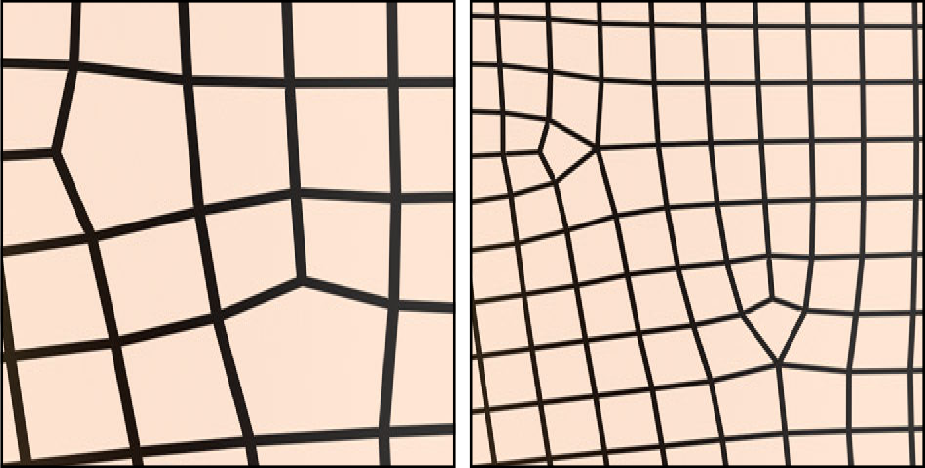
\includegraphics[width=9cm]{img/Singularities.png}\par
	\end{centering}
	\caption{Singularities create pentagons or triangles in quad-dominant mesh \textit{(left)}. Can be transformed into a pure-quad mesh through a subdivision step \textit{(right)}. \cite{jakob2015instant}}
	\label{fig:singularities}
\end{figure}

Since creating pure quad meshes is a difficult task, meshing algorithms oftentimes resort to quad-dominant meshes. \textbf{Quad-dominant meshes} are meshes, where the majority of faces are quadrilaterals and some are triangles or pentagons. Note however, that a quad-dominant mesh can be converted into a pure-quad mesh through a Catmull-Clark subdivision step (\cite{catmull1978recursively}) \cite{jakob2015instant}.\bigskip

When a tensor product structure is not needed, \textbf{triangle meshes} are often used because they have a smaller number of vertices per face in comparison to quad meshes, resulting in simplified geometric calculations. In addition, triangle-dominant meshes can be easily and efficiently converted into meshes of pure triangular faces, which are of course always flat. Because of these advantages, modeling a triangle mesh from data or even scratch can be much easier than modeling quad meshes. For example, most 3D scans produce triangle meshes, although often very non-uniform ones.\bigskip

\begin{figure}[htb!]
	\begin{centering}
		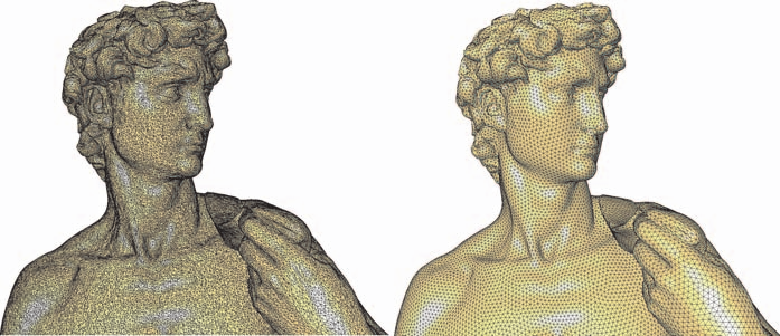
\includegraphics[width=9cm]{img/Uniform-Mesh.png}\par
	\end{centering}
	\caption{Nonuniform mesh \textit{(left)} and its uniform counterpart after uniform remeshing \textit{(right)}. \cite{alliez2008recent}}
	\label{fig:uniform-mesh}
\end{figure}

A mesh is \textbf{uniform} if its faces are as "uniform" as possible. This means the faces are of the same size. If a mesh is very non-uniform it is considered to be of higher complexity than a uniform replica. \textbf{Isotropy} is a property that describes uniformity in all directions. Thus, a uniform and isotropic mesh consists of equilateral triangles in triangle meshes or squares in quad meshes \cite{alliez2003isotropic,surazhsky2003isotropic}.

When modeling triangle meshes, it is not uncommon for the resulting meshes to be very non-uniform and have many redundant faces. Algorithms operating on triangle meshes may have great difficulty under such conditions. Therefore, it is of great advantage to simplify such meshes into uniform replicas and minimize the number of faces without losing the shape of the original geometry (Figure~\ref{fig:uniform-mesh}) \cite{jakob2015instant}.


\subsection{Global and local remeshing}\label{global-local-remeshing}
As mentioned earlier, many meshes are created using automated methods such as 3D scanning, which often results in poor quality meshes. For many geometry processing algorithms, these meshes are unsatisfactory and lead to performance and quality losses. Therefore, there is a need to reduce the complexity of these meshes, improve their quality, and sometimes even transform them into a completely different type of mesh. This process is referred to as \textbf{remeshing} \cite{alliez2008recent}.\bigskip

Although there are several central problems with all remeshing methods, one particularly complex problem is finding the appropriate location of a new vertex in the output mesh on the input surface. To deal with this, there are generally speaking two approaches: Either create an entirely new mesh for an output, or modify the input mesh to create the output mesh. Here, all remeshing methods are divided into two classes: Global remeshing and local remeshing, respectively \cite{botsch2007geometric,alliez2008recent}.\bigskip

\textbf{Global remeshing} solves the correspondence problem by creating a completely new mesh through parameterization of the input mesh. In mesh parameterization, a parametric equation is found for the surface of the mesh. Since the input and output meshes should represent the same surface, it is quite easy to find the corresponding position of a new vertex on the input mesh, provided that the parametric equation is known. Herein lies the major drawback of this global approach: determining the parametric equation of a surface is a challenge that can be, among other things, very computationally intensive and inaccurate. However, once the input mesh is successfully parameterized, a new high-quality mesh can be generated quite easily \cite{jakob2015instant,alliez2008recent}.

In summary, global remeshing techniques suffer from high time complexity and complex design, but can still provide high quality meshes. Some good approaches to this technique are the "Mixed-Integer Quadrangulation" algorithm by Bommes et al. (\cite{bommes2009mixed}) and "Periodic Global Parameterization" by Alliez et al (\cite{ray2006periodic}).\bigskip

On the other hand, there are \textbf{local remeshing} methods. These algorithms dispense with global mesh parameterization and instead work by modifying the initial mesh connectivity. Instead of creating a completely new initial mesh, local remeshing algorithms locally modify the input mesh itself by performing topological operations such as adding, moving, and removing vertices. By modifying the input mesh, the original surface is at least partially preserved in the output mesh, solving the correspondence problem. This process is highly scalable, robust, and simple. However, since the process is limited to local information around each vertex, it can lead to solutions that are not globally optimal. Therefore, local meshing processes are generally of lower quality than global meshing processes and also lead to mesh singularities due to their locality \cite{jakob2015instant,alliez2008recent}. The following parts of the paper briefly introduce the approach of \cite{tarini2010practical} and then compares it with the Instant Field-Aligned Meshes algorithm for field-aligned meshes.


\subsection{$N$-RoSy fields}\label{rosy}
The following described $N$-RoSy fields play an important role in many approaches to meshing surfaces, both global and local ones. In IFAM, $N$-RoSy fields are used to guide the orientation of edges in the output mesh \cite{jakob2015instant}.

In geometry, an $N$-way rotational symmetry is a property a shape has if it is invariant under rotations of a multiple of $\frac{2\pi}{N}$ about a point or an axis in 2D or 3D, respectively \cite{palacios2007rotational}. These symmetries can be thought of as vector fields, with $N$ vectors associated with each point, each pointing in a direction where the symmetry repeats (Figure~\ref{fig:n-rosy-singularities}). Hence, these symmetries are called $N$-way rotational symmetry fields (\textbf{$N$-RoSy fields}) \cite{panozzo2012fields}.

\begin{figure}[htb!]
	\begin{centering}
		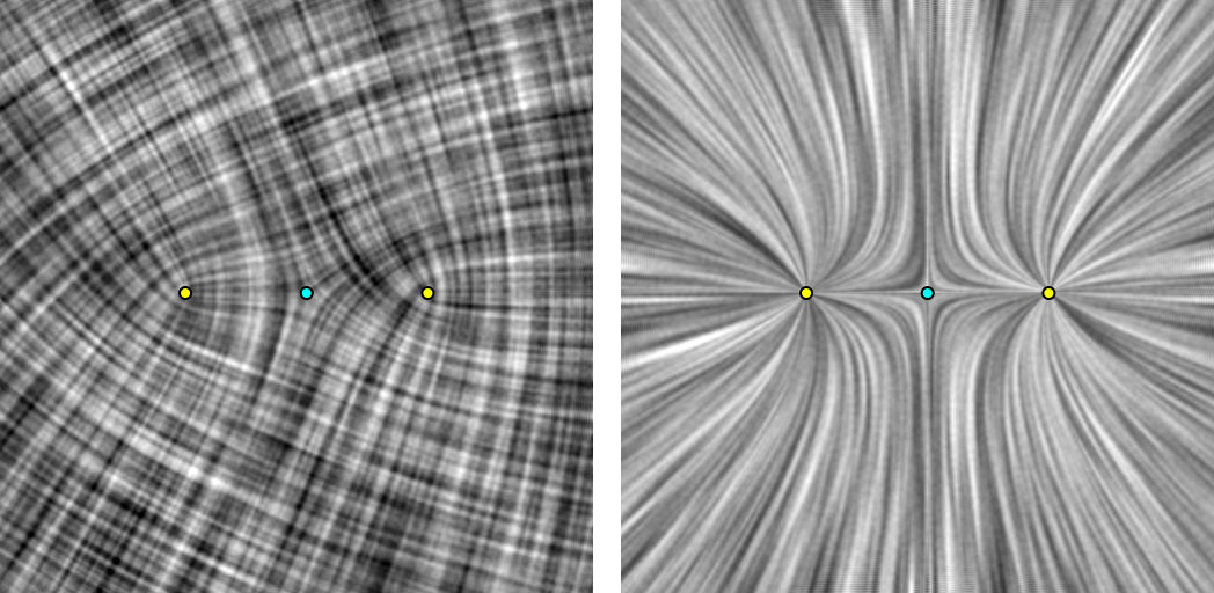
\includegraphics[width=9cm]{img/n-Rosy-Singularity.png}\par
	\end{centering}
	\caption{A comparison between a $4$-RoSy field \textit{(left)} and its representation vector field \textit{(right)}. In the $4$-RoSy field each point, excluding singularities, has $4$ different directional vectors that are invariant under rotation. This is visualized by lines forming crosses in the left field. As those directional vectors are invariant under rotation, the $4$-RoSy field can also be represented as a vector field, where each point has one representational directional vector. Notice how singularities (colored dots) are also of zero value in the vector field. \cite{palacios2007rotational}}
	\label{fig:n-rosy-singularities}
\end{figure}

Symmetries also occur on geometrical surfaces, where they are often defined as isometric automorphisms. This means, a surface can be mapped to itself while preserving all of its structure, i.e. distances and orientations. Symmetries can be categorized into two classes:
\begin{itemize}
	\item	\textbf{Intrinsic} symmetries preserve geodesic distances.
	\item	\textbf{Extrinsic} symmetries preserve euclidean distances.
\end{itemize}
In practice, though, geometries rarely have perfect symmetries on their entire surface. On most surfaces there are only local symmetries, and even they are not always ideal. Thus, deviations must be tolerated \cite{panozzo2012fields}.\bigskip

As a side effect of imperfect symmetries, $N$-RoSy fields introduce singularities. Note that these singularities can differ from singularities introduced in meshes. A singularity in an $N$-RoSy field is a point in the vector field where the associated vector is undefined (Figure~\ref{fig:n-rosy-singularities}) \cite{palacios2007rotational}. In short, they occur when the surface curves in a way that break the directions of the $N$-RoSy field. However, because of this property, they are also the points that control the topology of the field and thus the layout of the extracted mesh (Figure~\ref{fig:n-rosy-geometry}). Automatic generation of $N$-RoSy fields with optimal number and position of singularities remains a major challenge. Methods attempting this generally cannot operate without introducing new singularities that then appear as artifacts, such as irregular faces or vertices, on the extracted meshes \cite{lai2009metric}.

\begin{figure}[htb!]
	\begin{centering}
		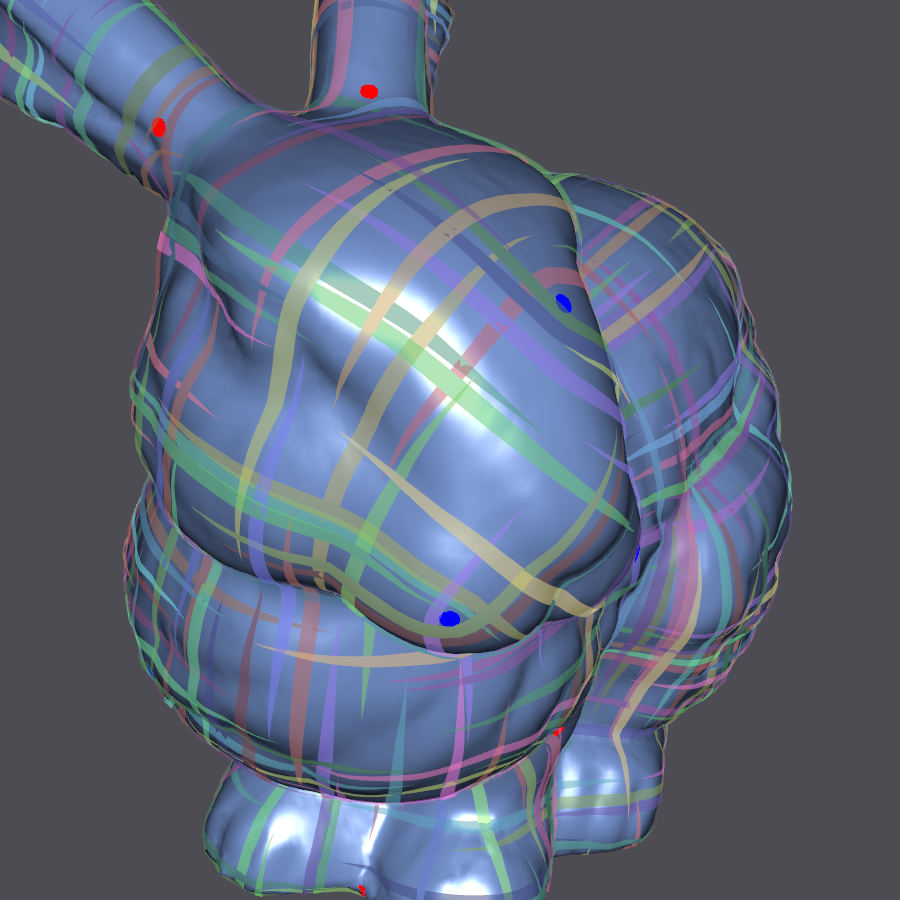
\includegraphics[width=5cm]{img/n-Rosy-orientation.png} 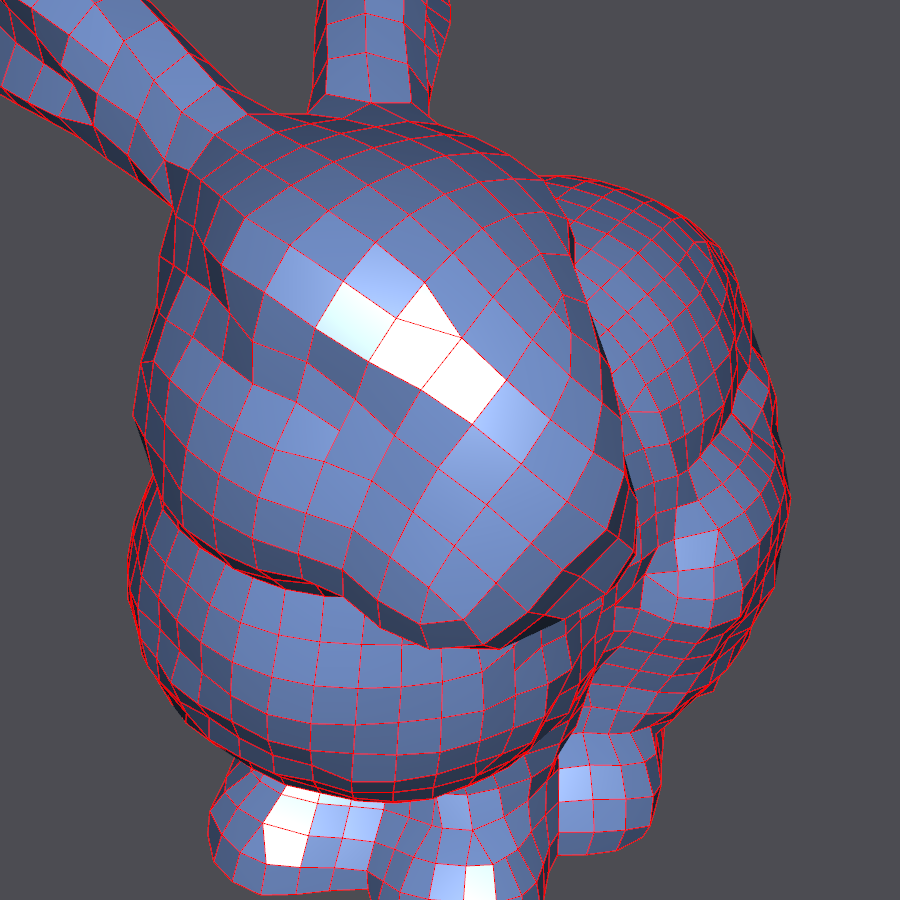
\includegraphics[width=5cm]{img/n-Rosy-Mesh.png}\par
	\end{centering}
	\caption{A $4$-RoSy orientation field calculated from a meshes surface \textit{(left)}. Note how singularities in the $4$-RoSy field (marked as colored dots), e.g. the singularity on the front right of the head, can introduce singularities or irregular vertices in the quad-dominant output mesh \textit{(right)}.}
	\label{fig:n-rosy-geometry}
\end{figure}



%%%%%%%%%%%%%%%%%%%%%%%%%%%%%%%%%%%%%%%%%%%%%%%%%%%%%%%%%%%%
% Related Work
\section{Related Work}\label{related_work}
The field of meshing surfaces is an ever advancing topic. Both global and local meshing methods are extensively researched in the past decades. More recently, since the advent of artificial intelligence, new data-driven approaches take on this challenging problem. Since there are many respectable studies in this area, this paper focuses its review on one approach from each technique, all of which generate quad-meshes. For a complete survey, the reader is referred to \cite{bommes2013quad}.

\subsection*{Mixed-Integer Quadrangulation.}\label{MIQ}
Mixed-Integer Quadrangulation (\textit{MIQ}) by \cite{bommes2009mixed} is a global method for remeshing given triangle meshes into quad-meshes. The goal of this method is to create a global mesh parameterization (Section~\ref{global-local-remeshing}), which can then be used to extract a quad mesh.\bigskip

Similar to the Instant Field-Aligned Meshes approach, MIQ first creates an orientation field on the mesh. This is done by assigning a direction to each triangle face and then aligning them at 90 degree angles, since the resulting mesh should be a quad mesh, and finally smoothing out the field. Creating such a smooth cross field is mathematically challenging. The authors suggest formulating this problem as a mixed-integer optimization problem, which then can be solved using a mixed-integer programming solver. Afterward, this smooth cross field can be used to cut the triangle mesh and unfold it into a 2D plane, allowing for a global mesh parameterization. Finally, this global parameterization can be used to extract a quad mesh that lies on top of the 2D plane, which can then lift back into 3D \cite{bommes2009mixed,schmidt2014towards}.

\subsection*{Practical quad mesh simplification.}\label{PQMS}
Practical quad mesh simplification (\textit{PQMS}) by \cite{tarini2010practical} is a local method to generating quad meshes with low complexity, starting from high-complexity ones. Its goal is to globally maximize the tessellation quality, i.e. to reduce the number of irregular vertex valencies. Note that mesh simplification is a related, but still different topic to remeshing. Mesh simplification is not necessarily about improving the overall quality of the mesh, but about reducing the complexity, which is fundamentally not the case for remeshing algorithms.\bigskip

PQMS operates based on crucial observation: An ideal quad mesh with  zero complexity consists entirely of flat, equilateral, regular, uniform squares. Such a mesh has the property that all edges have the same length $l$, and all diagonals of each face are of length $l \sqrt{2}$ \cite{tarini2010practical}.

The authors can approximate such a mesh by local rule-based optimization operations on adjacent quad faces. Local smoothing operations include rotations of vertices/edges and collapsing of edges/diagonals. For each set of neighboring faces, these operations are prioritized according to their contribution to improving the tessellation quality of the mesh \cite{tarini2010practical}.

\subsection*{Data-Driven Interactive Quadrangulation.}\label{DDIQ}
A fairly new approach to the meshing problem is machine learning. The Data-Driven Interactive Quadrangulation method (\textit{DDIQ}) by \cite{marcias2015data} can interactively quadrangulate user-sketched patches in geometries. Similar to previous approaches, DDIQ also follows a pattern-based quadrangulation model: Starting from a patch on the surface, i.e. a part not yet meshed, a quad mesh is filled in based on a certain pattern. This pattern is adaptable to the boundary constraints of the patch, i.e. the edges of the surrounding mesh. The pattern can be selected from a database of possible patterns based on how well it quadrangulates the patch \cite{marcias2015data}.

Unlike previous work, DDIQ does not rely on only a few predefined patterns: This approach can automatically analyze patterns in already existing quad meshes, which can of course be used to create new meshes. In this way, a large database of patterns can be learned from numerous meshes manually designed by artists. The appropriate patterns can then be selected based on user-defined topological and geometrical criteria. As a result, the quality of the filled patches increases with the number of analyzed patterns \cite{marcias2015data}.


%%%%%%%%%%%%%%%%%%%%%%%%%%%%%%%%%%%%%%%%%%%%%%%%%%%%%%%%%%%%
% Main Sections
\section{Method}\label{algorithm}
A new local remeshing approach is the Instant Field-Aligned Meshes algorithm (\textit{IFAM}). The pipeline described below is very simple to implement and time efficient.

Basically, it takes a graph representation of the geometry's surface as an input and outputs either a triangle-based or a quad-dominant isotropic mesh. To create this mesh, the algorithm computes two fields based on the input graph, the orientation- and position-field, respectively, of which the first one is an $N$-RoSy field (Section~\ref{rosy}). To globally align the mesh with a direction field, the orientation- and position-field are then iteratively optimized through local smoothing operations, either intrinsic or extrinsic. The output mesh can then be extracted from both fields \cite{jakob2015instant}.

% Input
\subsection{Input representation}
As mentioned before, the algorithm takes as input the surface of the geometry represented as a graph $\mathcal{G} = (\mathcal{V}, \mathcal{E})$. Each element $i \in \mathcal{V}$ is called a vertex and represents a position $v_i \in \mathbb{R}^3$ and a normal direction $n_i \in \mathbb{R}^3$ on the surface. $\mathcal{E} \subseteq \mathcal{V} \times \mathcal{V}$, also called the set of edges, stores neighboring vertices in the graph. It is defined differently depending on the original geometric representation:
\begin{itemize}
	\item	For meshes, $\mathcal{E}$ is equal to the usual set of edges in the mesh.
	\item	For point clouds, $(i,j) \in \mathcal{E}$ if the vertex $i$ is in the set of $K$-nearest neighbors by distance of $j$.
\end{itemize}
The neighborhood of a vertex $i$ is denoted by $\mathcal{N}(i) = \{j \in \mathcal{V} \mid (i,j) \in \mathcal{E}\}$. Additionally, weights $w_{ij}$ can be assigned to each edge $(i,j) \in \mathcal{E}$. These weights affect the subsequent smoothing of the orientation- and position-field and can be chosen geometry-dependent or uniform (equal to $1$). They will be used in the following optimization pipelines \cite{jakob2015instant}.\bigskip

This simple input representation allows the use of many geometry representations in this algorithm, as long as one can convert them into the described graph input format.

% Fields
\subsection{Fields}
Based on the input graph, the algorithm now computes an $N$-RoSy field parameter-free. This field, which is called the \textbf{orientation field}, represents a set of directions on the input geometry along which the edges of the output mesh should align. To compute this step, the algorithm locally optimizes a smoothness energy of the field, which will be defined in the following, to either respect geodesic distances (\textbf{intrinsic}) or to automatically snap to the edges of the geometry (\textbf{extrinsic}). Afterward, this orientation field is used to calculate a positional symmetry field (PoSy field, or \textbf{position field}). Using integer translations, a parameterization is calculated locally for each vertex, and its gradient is set to be aligned to the orientation field. Then, the algorithm also minimizes this fields smoothness energy, again either intrinsic or extrinsic \cite{jakob2015instant}.\bigskip

Only few user-defined parameters are required for the following mechanisms:
\begin{itemize}
	\item	Whether the output mesh should be a triangle mesh or a quad-dominant mesh: $s_o = 6$ or $s_o = 4$, respectively.
	\item	The desired edge length $\rho$ in the output mesh.
	\item	Whether the fields should be calculated intrinsically or extrinsically.
\end{itemize}

\subsubsection{Orientation field}\label{orientation-field}
The first step of the algorithm computes an $s_o$-RoSy field (Section~\ref{rosy}), which is called the \textbf{orientation field}. This field is used to align the edges in the output mesh.\bigskip

Briefly, to compute this orientation field, one needs to determine all integer rotations of the vertices/edges in our input graph $\mathcal{G}$ and then smooth the neighboring directions in the resulting field. This process, which will be described in detail in the following sections, is heavily inspired by the works of \cite{bommes2009mixed,ray2008n}, however works completely locally and is thus much simpler in design, while still giving comparable results \cite{jakob2015instant}.

\begin{wrapfigure}{r}{3cm}
	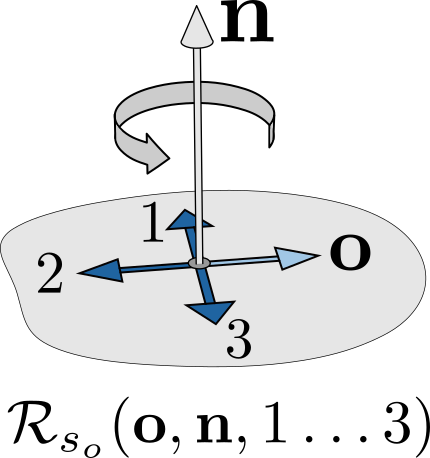
\includegraphics[width=3cm]{img/integer-rotation.png}\par
	\label{fig:integer-rotation}
\end{wrapfigure}

\paragraph{Symmetry group.}
Depending on its type, in the (isotropic) output mesh, each vertex has 3 or 4 directions, which the edges face in. They will be aligned by this orientation field, which is calculated only using the input graph $\mathcal{G}$. For that, the algorithm first needs to assign to each $i \in \mathcal{V}$ a \textit{representative} direction $o_i \in \mathbb{R}^3$. The initial value of $o_i$ does only minimally affect the final result, as it is used to create integer rotations around the normal direction $n_i$ of vector $i$ and will be optimized.\bigskip

The authors denote the rotation matrix by angle $\theta$ about vector $n$ as $\rot(n, \theta)$. Now, an integer rotation of a representative vector $o$ about a fixed normal $n$ can be expressed as $\mathcal{R}_{s_o}(o,n,k)$, and the set of all integer rotations of $o$ about $n$ as $\mathcal{R}_{s_o}(o,n)$:
\begin{equation*}
\begin{split}
	& \mathcal{R}_{s_o}(o,n,k) \coloneqq \rot \left(n, k \cdot \frac{2\pi}{s_o} \right) o, \quad k \in \mathbb{Z} \\
	& \mathcal{R}_{s_o}(o,n) \coloneqq \{\mathcal{R}_{s_o}(o,n,0), \dots, \mathcal{R}_{s_o}(o,n,s_o-1)\}
\end{split}
\end{equation*}
Thus, before any optimization is done, the orientation field consists of all the directions in $\mathcal{R}_{s_o}(o_i, n_i)$ for every vertex $i \in \mathcal{V}$.

\begin{figure}[htb!]
	\begin{centering}
		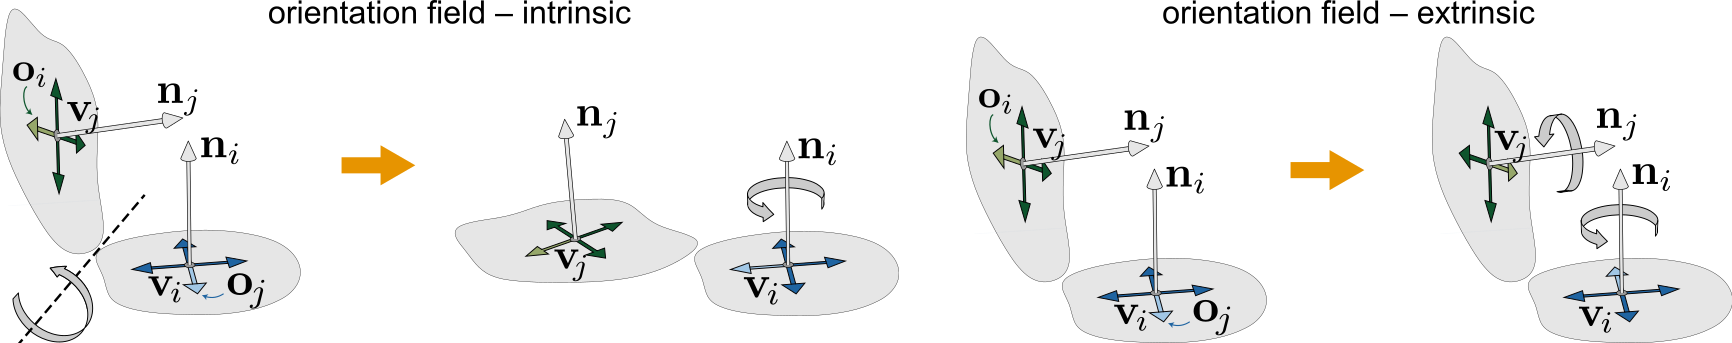
\includegraphics[width=\textwidth]{img/orientation-field-intrinsic-extrinsic-horizontal.png}\par
	\end{centering}
	\caption{Optimizing the smoothness of the orientation $s_o$-RoSy field intrinsically \textit{(left)} and extrinsically \textit{(right)}. \cite{jakob2015instant}}
	\label{fig:orientation-field-intrinsic-extrinsic}
\end{figure}

\paragraph{Intrinsic smoothness.}
As mentioned earlier, the authors based their methods on the work of \cite{ray2008n,bommes2009mixed}. Here, they propose to minimize the smoothness energy of an $N$-RoSy field by smoothening out the angular difference between adjacent vectors. For this, vectors are being folded into a common plane (Figure~\ref{fig:orientation-field-intrinsic-extrinsic}, top), which preserves the intrinsic properties of the surface while also making the angular differences easier to compute \cite{jakob2015instant}.\bigskip

Since each vertex has $s_o$ representative direction vectors, the authors encode this matching through integer variables $k_{ij} \in \mathbb{Z}$ for each edge $(i,j) \in \mathcal{E}$ and store them in a vector $k \in \mathbb{Z}^{2 \vert \mathcal{E} \vert}$.

The smoothness energy of the entire $s_o$-RoSy field $O$ can now be calculated as:
\begin{equation}\label{eq:orientation-isotropic-energy}
	E_i(O,k) \coloneqq \sum_{i \in \mathcal{V}} \sum_{j \in \mathcal{N}(i)} \angle(o_i, \mathcal{R}_{s_o}(o_{ji}, n_i, k_{ij}))^2,
\end{equation}
where $o_{ji}$ is the representative vector $o_j$ at vertex $j$, folded into the tangent plane of vertex $v_i$. It is defined as the following:
\begin{equation*}
	o_{ji} \coloneqq \rot(n_j \times n_j, \angle(n_j, n_i))o_j
\end{equation*}
A low smoothness energy leads to a more uniform, isotropic and higher quality output mesh. So it is the goal to minimize this energy. In order to do so, one must find optimal values for each $o_i$ and $k_{ij}$ \cite{jakob2015instant}.\bigskip

While \cite{bommes2009mixed} proposed to minimize the smoothness energy globally, the approach IFAM follows is a local optimization using iteration over all vertices in $\mathcal{V}$. Hence, this approach is a lot less complex than global ones, while still yielding comparable results.

Whenever the iteration visits the vertex $i$, the algorithm first determines optimal integer variables $k_{ij}$ by a brute-force search:
\begin{equation}\label{eq:orientation-intrinsic-integer}
	k_{ij} \coloneqq \argmin_{0 \leq k' < s_o} \angle(o_i, \mathcal{R}_{s_o}(o_{ji}, n_i, k'))
\end{equation}
In this way, the algorithm can already find improved values for $\mathcal{R}_{s_o}(o_{ji}, n_i, k_{ij})$ in the smoothness energy equation \eqref{eq:orientation-isotropic-energy}.

Furthermore, the representative direction vector $o_i$ can be optimized, i.e. rotated, by:
\begin{equation}\label{eq:orientation-intrinsic-vector}
\begin{split}
	& o_i \leftarrow \sum_{j \in \mathbb{N}(i)} w_{ij} \cdot \mathcal{R}_{s_o}(o_{ji}, n_i, k_{ij})\\
	& o_i \leftarrow \frac{o_i}{\Vert o_i \Vert}
\end{split}
\end{equation}
Here, the weighing $w_{ij}$ of edges can be used to guide the orientation field in certain directions at certain locations \cite{jakob2015instant}.\bigskip

However, the authors have found that this process can be significantly improved if the integer variables $k_{ij}$ are recomputed after visiting each edge. Thus, we can improve the process \eqref{eq:orientation-intrinsic-vector}:
\begin{equation}
\begin{split}
	& o_i' \leftarrow w_{ij_1} \cdot \mathcal{R}_{s_o}(o_{j_1i}, n_i, k_{ij_1}), \qquad o_i \leftarrow \frac{o_i'}{\Vert o_i' \Vert}\\
	& \textrm{recompute all } k_{ij}\\
	& o_i' \leftarrow o_i' + w_{ij_2} \cdot \mathcal{R}_{s_o}(o_{j_2i}, n_i, k_{ij_2}), \qquad o_i \leftarrow \frac{o_i'}{\Vert o_i' \Vert}\\
	& \textrm{recompute all } k_{ij}\\
	& \dots
\end{split}
\end{equation}
where $j_1, j_2, \dots \in \mathcal{N}(i)$.

\paragraph{Extrinsic smoothness.}
This intrinsic calculation has a disadvantage: Two vectors are always folded into a common plane. While this is efficient, it often loses desirable information about the curvature of the geometry. This behavior is illustrated in Figure~\ref{fig:orientation-field-illustration}. The authors' proposed alternative, which is also parameter-free, can naturally align with edges in the geometry. They achieve this by not folding two vectors into a common plane, but rather leaving them in embedded space \cite{jakob2015instant}.\bigskip

To do so, we must apply some modifications to the previous formulas:
The extrinsic smoothness formula is now:
\begin{equation}\label{eq:orientation-extrinsic-energy}
	E_e(O,k) \coloneqq \sum_{i \in \mathcal{V}} \sum_{j \in \mathcal{N}(i)} \angle(\mathcal{R}_{s_o}(o_{i}, n_i, k_{ij}), \mathcal{R}_{s_o}(o_{j}, n_j, k_{ji}))^2,
\end{equation}
The brute force search from equation \eqref{eq:orientation-intrinsic-integer} now changes to the following:
\begin{equation}\label{eq:orientation-extrinsic-integer}
	(k_{ij}, k_{ji}) \coloneqq \argmin_{0 \leq k',k'' < s_o} \angle(\mathcal{R}_{s_o}(o_i, n_i, k'), \mathcal{R}_{s_o}(o_j, n_j, k''))
\end{equation}
Finally, we can also adapt the algorithm to optimize $o_i$ and its iterative improvement \eqref{eq:orientation-intrinsic-vector} to fit these conditions in a similar fashion \cite{jakob2015instant}.

\begin{figure}[htb!]
	\begin{centering}
		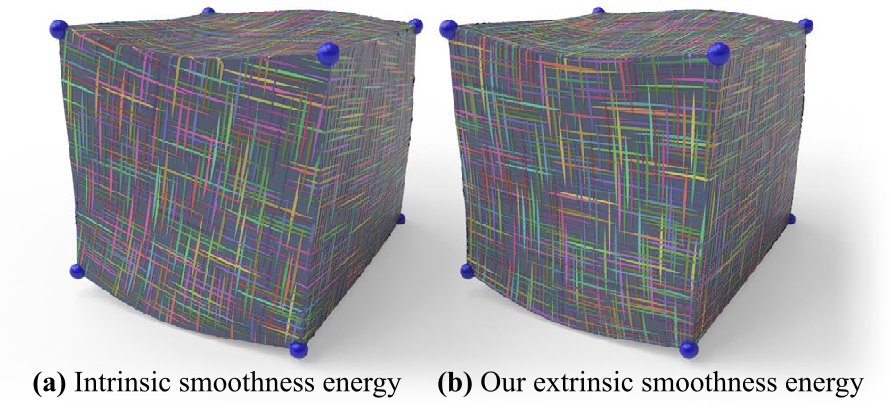
\includegraphics[width=8cm]{img/orientation-field-illustration.png}\par
	\end{centering}
	\caption{Orientation fields after optimizing the smoothness energy intrinsically \textit{(left)} and extrinsically \textit{(right)}. \cite{jakob2015instant}}
	\label{fig:orientation-field-illustration}
\end{figure}

\paragraph{Singularities.}
Since the orientation field is an $N$-RoSy field, singularities can naturally occur (Section~\ref{rosy}). The singularities in an orientation field do affect the orientation of points in that specific location, but in the output mesh only correspond to irregular vertices \cite{jakob2015instant}.

\subsubsection{Position field}
Now that the algorithm has created and optimized the $s_o$-RoSy orientation field $O$, it can move on to the next step, which is computing the \textbf{position field}. By design, this field is perfectly aligned with the orientation field and will specify the location of vertices on the output mesh \cite{jakob2015instant}.\bigskip

This calculation is also based on the works of \cite{bommes2009mixed} and \cite{ray2006periodic}. In order to create such a position field, it has been proposed in previous methods to compute a global parameterization of the entire surface. This would allow the surface to be mapped into 2 dimensions ($(u,v)$-parameterization), then a grid of triangles or quadrilaterals to be placed on that plane, and finally the mesh to be lifted back into 3-dimensional space. However, such global algorithms are complex to implement, very sensitive to topological noise, and, most importantly, do not scale well with the size of the input graph \cite{jakob2015instant}.\bigskip

This algorithm addresses the same problem again through a local solution: It computes a local parameterization for each vertex instead of finding a continuous parameterization function for the entire mesh. Similar to the orientation field, the algorithm then locally minimizes the smoothness energy between neighboring local parameterizations. More precisely, the smoothness between two such local parameterizations refers to the similarity between them in regard to integer translations \cite{jakob2015instant}.

\begin{wrapfigure}{r}{3cm}
	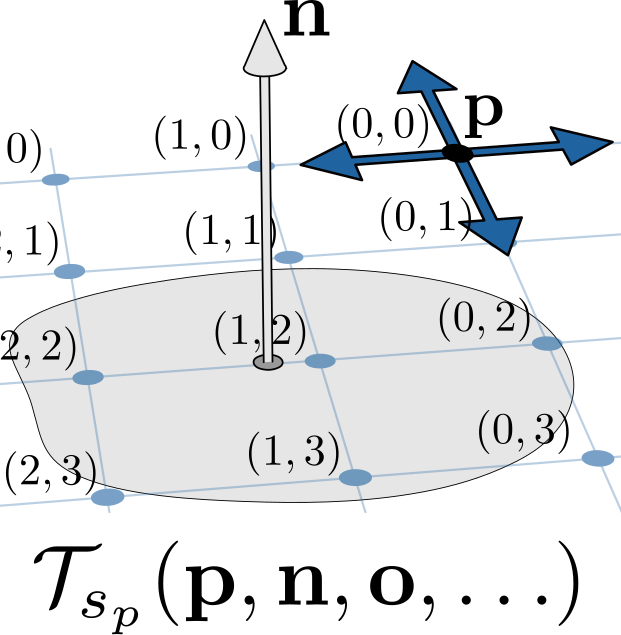
\includegraphics[width=3cm]{img/integer-translation.png}\par
	\label{fig:integer-translation}
\end{wrapfigure}

\paragraph{Symmetry group.}
The authors propose a simple yet efficient encoding for the local parameterization of a vertex $i$: The parameterization's gradient is set to be exactly aligned with the orientation field $o_i$ (Section~\ref{orientation-field}).

Since the gradient is fixed by $o_i$, one can then encode the local parameterization of vertex $i$ in a point $p_i \in \mathbb{R}^3$. \cite{jakob2015instant} proposes this point $p_i$ to be the closest lattice point to $v_i$.

Let $s_p = m \cdot s_o, m \in \mathbb{N}$. The local parameterization is, of course, invariant under rotations by integer multiples of $\frac{2\pi}{s_p}$ (Section~\ref{rosy}). But more importantly, it is invariant under integer translations of $\rho$ along the $s_p$ symmetry axes \cite{jakob2015instant}.\bigskip

Let $s_p$ be even. Integer translations of a position $p \in \mathbb{R}^3$ about $\rho$ and the set of all its possible integer translations are defined as:
\begin{equation*}
\begin{split}
	& \mathcal{T}_{s_p}(p,n,o,t) \coloneqq p + \rho \cdot \sum_{k=0}^{\frac{s_p}{2}-1} t_k \mathcal{R}_{s_p}(o,n,k)\\
	& \mathcal{T}_{s_p}(p,n,o) \coloneqq \left\{\mathcal{T}_{s_p}(p,n,o,t) \mid t \in \mathbb{Z}^{\frac{s_p}{2}}\right\}.
\end{split}
\end{equation*}
Since $s_p$ is even, the sum over $\frac{s_p}{2}$ terms ensures that each orientation- (or rather translation-) axis is considered once. Each integer $t_k$ then translates $p$ by $\rho$ units in the respective axis.

Given the local parameterization for each vertex, the position field $P$ can now be defined as the set of all integer translations $\mathcal{T}_{s_p}(p_i, n_i, o_i)$ from each vertex $i$ \cite{jakob2015instant}.

\paragraph{Intrinsic smoothness.}
Similar to the orientation field, we again introduce new integer variables due to the ambiguity of symmetry: For each edge $(i,j) \in \mathcal{E}$, there is an integer vector $t_{ij} \in \mathbb{Z}^{\frac{s_p}{2}}$ representing integer jumps in the integer translation. For the sake of simplicity, we again store these variables in a vector $t$.\bigskip

The intrinsic smoothness energy of the position field $P$ can now be measured as:
\begin{equation*}
	E_i(P,t) \coloneqq \sum_{i \in \mathcal{V}} \sum_{j \in \mathcal{N}(i)} \Vert p_i - \mathcal{T}_{s_p}(p_{ji}, n_i, o_i, t_{ij}) \Vert ^2_2
\end{equation*}
$p_{ji}$ represents $p_j$ of vertex $j$ after being rotated into the tangent plane of $v_i$. It is defined as follows:
\begin{equation*}
	p_{ji} \coloneqq \rot(n_j \times n_i, \angle(n_j, n_i)) (p_j - q_{ij}) + q_{ij}
\end{equation*}
$q_{ij}$ is the point that intersects the tangent planes of both $v_i$ and $v_j$, while also having minimum distance to both points. Since this approach is intrinsic, $q_{ij}$ simply becomes the midpoint of $v_i$ and $v_j$, after both are rotated into the same plane.\bigskip

Again, to minimize the smoothness energy, one must optimize the values for each $p_i$ and $t_{ij}$. The algorithm does this in a very similar fashion to the approach used in the optimization of the orientation field. Although this can be done intrinsically, because of the often undesired properties of intrinsic algorithms, we will focus on the extrinsic optimization. As with the orientation field, the intrinsic and extrinsic approaches differ in that the vectors are not rotated into another plane, but are left in three-dimensional space. For further information on the intrinsic approach, the reader is referred to \cite{jakob2015instant}.

\begin{figure}[htb!]
	\begin{centering}
		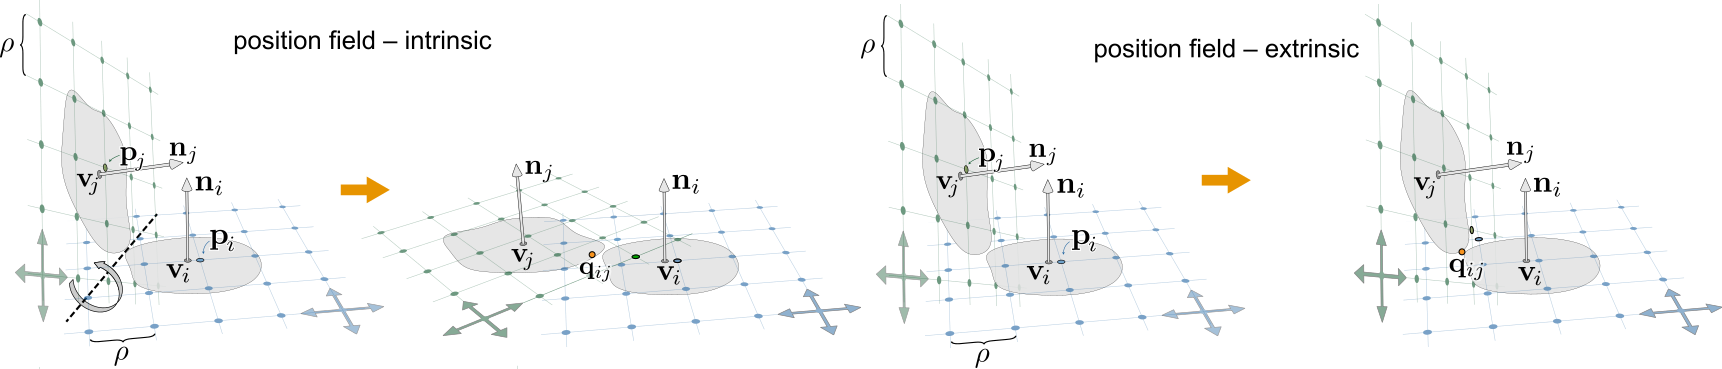
\includegraphics[width=\textwidth]{img/position-field-intrinsic-extrinsic-horizontal.png}\par
	\end{centering}
	\caption{Optimizing the smoothness of the position field intrinsically \textit{(left)} and extrinsically \textit{(right)}. \cite{jakob2015instant}}
	\label{fig:position-field-intrinsic-extrinsic}
\end{figure}

\paragraph{Extrinsic smoothness}
When the smoothness energy is optimized extrinsically, one first has to determine $q_{ij}$. In the intrinsic approach, it could be defined as the midway between two vertices. In the extrinsic approach, $q_{ij}$ still must minimize the distance to $v_i$ and $v_j$, however also maintain its position on both their respective tangent planes. This is constrained least-squares problem has a simple solution:
\begin{equation*}
\begin{split}
	& q_{ij} \coloneqq \frac{1}{2}(v_i + v_j) - \frac{1}{4}(\lambda_i n_i + \lambda_j n_j),\\
	& \lambda_i \coloneqq \frac{2 \langle (n_i + \langle n_i, n_j \rangle n_j, v_j - v_i \rangle)}{1 - \langle n_i, n_j \rangle ^2 + \epsilon}
\end{split}
\end{equation*}
where $\epsilon > 0$ is small real number ensuring a reasonable value for $n_i = n_j$ \cite{jakob2015instant}.\bigskip

With this position in hand, one can now optimize the integer jumps $t_{ij}$ through brute-force search over a fairly minimal set:
\begin{equation*}
	(t_{ij}, t_{ji}) \coloneqq \argmin_{t' \in Q_{ij}, t'' \in Q_{ji}} \Vert \mathcal{T}_{s_p}(p_i, n_i, o_i, t') - \mathcal{T}_{s_p}(p_j, n_j, o_j, t'') \Vert
\end{equation*}
where sets $Q_{ij}$ and $Q_{ji}$ contain the $s_p$ closest integer translations of $q_{ij}$ to $q_{ij}$ and $q_{ji}$ to $q_{ji}$ respectively \cite{jakob2015instant}.\bigskip

Using this, each of the vertices representative position $p_i$ can now be optimized using the following iterative algorithm, similar to the orientation field optimization:
\begin{equation*}
\begin{split}
	& p_i' \leftarrow w_{ij_1} \mathcal{T}_{s_p}(p_{j_1i}, n_i, o_i, t_{ij_1}), \qquad p_i \leftarrow \frac{p_i'}{\sum_{k=1}^1 w_{ij_k}} \\
	& \textrm{recompute all } t_{ij}\\
	& p_i' \leftarrow p_i' + w_{ij_2} \mathcal{T}_{s_p}(p_{j_2i}, n_i, o_i, t_{ij_2}), \qquad p_i \leftarrow \frac{p_i'}{\sum_{k=1}^2 w_{ij_k}} \\
	& \textrm{recompute all } t_{ij}\\
	& \dots
\end{split}
\end{equation*}
where $j_1, j_2, \dots \in \mathcal{N}(i)$ \cite{jakob2015instant}.

\begin{figure}[htb!]
	\begin{centering}
		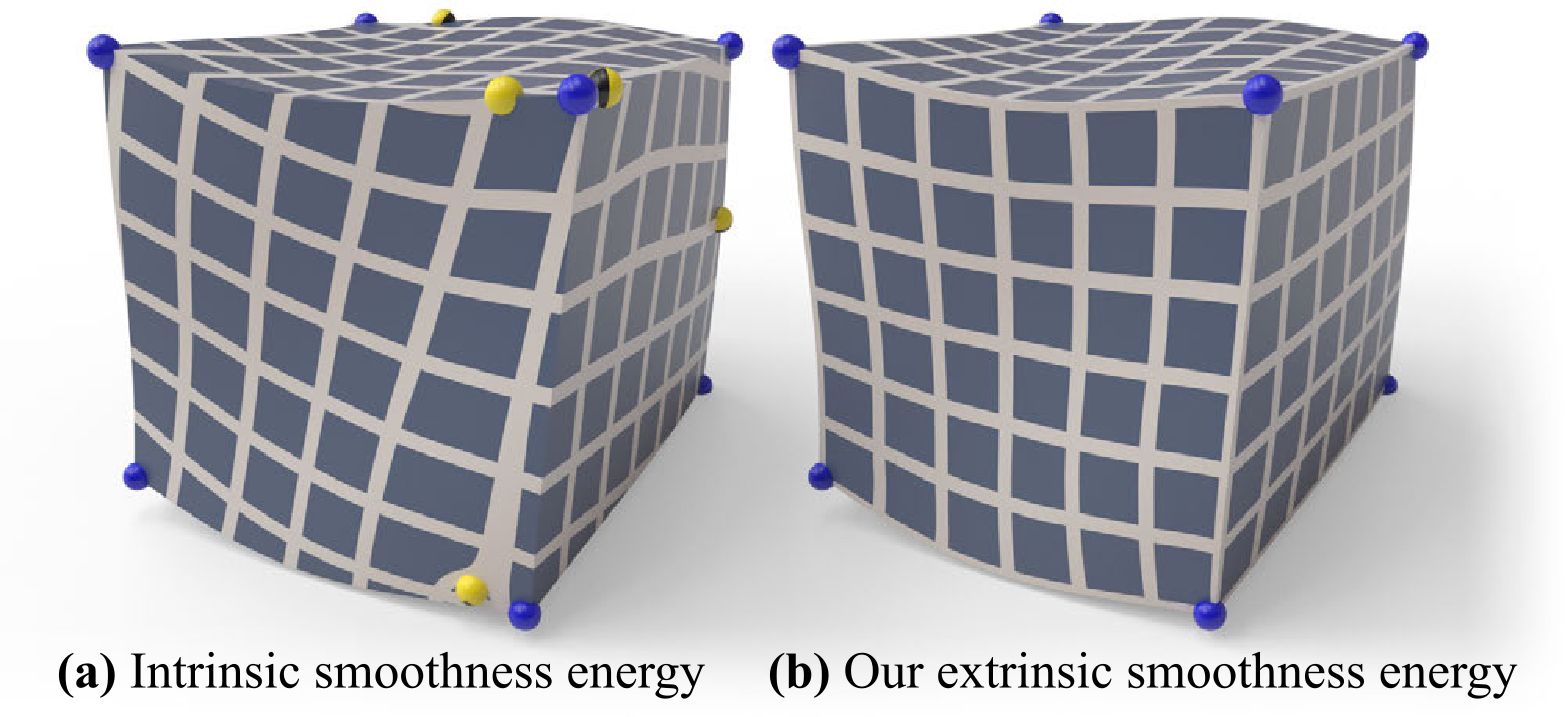
\includegraphics[width=8cm]{img/position-field-illustration.png}\par
	\end{centering}
	\caption{Position fields after optimizing the smoothness energy intrinsically \textit{(left)} and extrinsically \textit{(right)}. \cite{jakob2015instant}}
	\label{fig:position-field-illustration}
\end{figure}

\paragraph{Singularities.}
With this localized approach, singularities can also occur in position fields. Here they correlate to residual integer translations over a cycle and are not defined if an orientation singularity is already present at that location. Similar to orientation field singularities, position singularities result in an irregular vertex. However, in quad-dominant meshes, they can also produce T-junctions instead of irregular vertices \cite{jakob2015instant}.

% Multiresolution hierarchy
\subsection{Multiresolution hierarchy}
\begin{figure}[htb!]
	\begin{centering}
		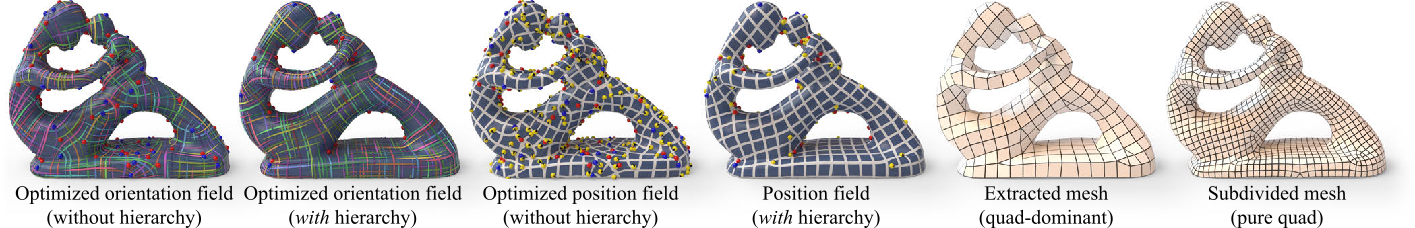
\includegraphics[width=\textwidth]{img/multiresolution-hierarchy.png}\par
	\end{centering}
	\caption{The iterations used in the orientation- and position-field optimizations can locally smooth their respective fields. However, they tend to get stuck in local minima. Multiresolution hierarchy is able to minimize this problem, resulting in smoother fields and fewer singularities. \cite{jakob2015instant}}
	\label{fig:multireolution-hierarchy}
\end{figure}

The main drawback of the iterations used in both orientation- and position-field optimization is that they can get stuck in local minima. This happens when multiple nearby vertices have very similar properties and the iteration looping over the graphs vertices visits these vertices right after one another. Then, if in the internal optimization iterations (e.g. algorithm \eqref{eq:orientation-intrinsic-vector}) those vertices are visited in the beginning and right after one another, it can, to a certain extent, fix these properties. Visiting other edges without similar properties afterward can then have little to no effect on those properties. Properties stuck in local minima create artifacts in the respective fields that do not follow the geometry's surface \cite{jakob2015instant}.\bigskip

A really simple approach to this problem is to generate a random permutation of the vertices every time a vertex $i$ is visited.

The authors however propose the use of an optional preprocessing step called \textbf{multiresolution hierarchy}. In short, it repeatedly collapses neighboring vertices into "super-vertices". A more detailed scheme is:
\begin{enumerate}
	\item	Processing: assign a value $A_i = 1$ to each vertex $i \in \mathcal{V}$.
	\item	Repeat, until no collapses are possible:
			\begin{enumerate}
				\item	For each edge $(i,j) \in \mathcal{E}$ assign a score:
						\begin{equation*}
							S_{ij} \coloneqq \langle n_i, n_j \rangle \cdot \min\left(\frac{A_i}{A_j}, \frac{A_j}{A_i}\right)
						\end{equation*}
				\item	Iterate over $S_{ij}$ decreasingly and collapse vertices $i,j$ into the new vertex $v$, only if neither has been collapsed yet.\\
						The new vertex is assigned an area of $A_v = A_i + A_j$, its other properties are determined by the area-weighted areas of all the merged vertices in $v$.
			\end{enumerate}
\end{enumerate}
The exact process is described in more detail by \cite{jakob2015instant}, which also takes inspiration from \cite{botsch2006primo}. This method can be reapplied multiple times (multiple depths), resulting in different results (Figure~\ref{fig:multireolution-hierarchy-depths}).

\begin{figure}[htb!]
	\begin{centering}
		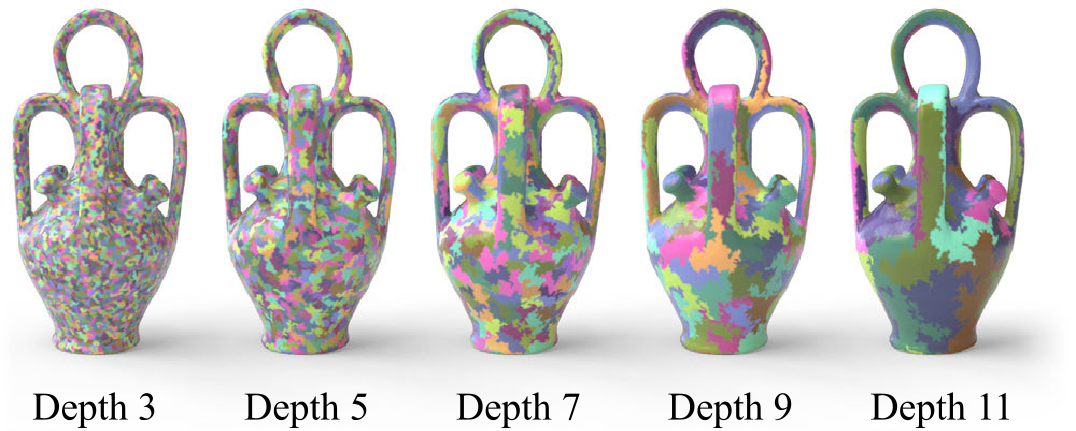
\includegraphics[width=8cm]{img/multiresolution-hierarchy-depths.png}\par
	\end{centering}
	\caption{An illustration of the position field after the application of multiresolution hierarchy at various depths. Notice how extreme depth values can result in lower quality results. \cite{jakob2015instant}}
	\label{fig:multireolution-hierarchy-depths}
\end{figure}

% Exporting
\subsection{Mesh extraction}
After the algorithm has created and optimized the orientation- and position-field and thus also modified the properties of the vertices in the input graph $\mathcal{G}$, an output mesh can finally be extracted. To do so, the proposed algorithm takes an intermediate step and computes a new undirected graph $\mathcal{G}' = (\mathcal{V}', \mathcal{E}')$. Let $\mathcal{V}' = \{p_i \mid i \in \mathcal{V}\}$, and connect two vertices $(i,j)$ if $t_{ij}$ is unit vector-valued. These types of unit vector-valued integer jumps are particularly interesting, since they state that $p_i$ and $p_j$ are just a single integer translation apart, thus approximating edges in the output mesh. Moreover, let $\mathcal{C} \coloneqq \{(i,j) \in \mathcal{E} \mid t_{ij} = -t_{ji}\}$. The edges in $\mathcal{C}$ have integer values that reference the same point by integer translation \cite{jakob2015instant}.

We can now iterate over the edges $(i,j) \in \mathcal{C}$ in ascending order of the distance $\Vert p_i - p_j \Vert$ and add those edges to $\mathcal{E}$ if neither $i$ nor $j$ are already connected by an edge. This filtering process is beneficial to the quality of the output mesh since it avoids collapsing vertices too eagerly near orientation- and position-field singularities. Further filtering and optimization operations can be applied, as described in \cite{jakob2015instant}.\bigskip

Finally, the output mesh can be extracted from $\mathcal{G}'$, which now contains position and adjacency information. All that remains is to detect faces in $\mathcal{G}'$, which can be done using a simple greedy algorithm. However, this approach is error-prone to harsh conditions, and can produce non-manifold outputs. To still produce manifold outputs, one can simply remove problematic vertices and edges from $\mathcal{G}'$. Note that this will still produce local artifacts in the output mesh restricted to the regions of the original non-manifold sub-meshes \cite{jakob2015instant}.

%%%%%%%%%%%%%%%%%%%%%%%%%%%%%%%%%%%%%%%%%%%%%%%%%%%%%%%%%%%%
% Results
\section{Results and Discussion}\label{results}
The simplicity and locality of operations in the Instant Field-Aligned Meshes method lead to incredible scalability, efficiency, and robustness compared to global approaches.

\begin{figure}[htb!]
	\begin{centering}
		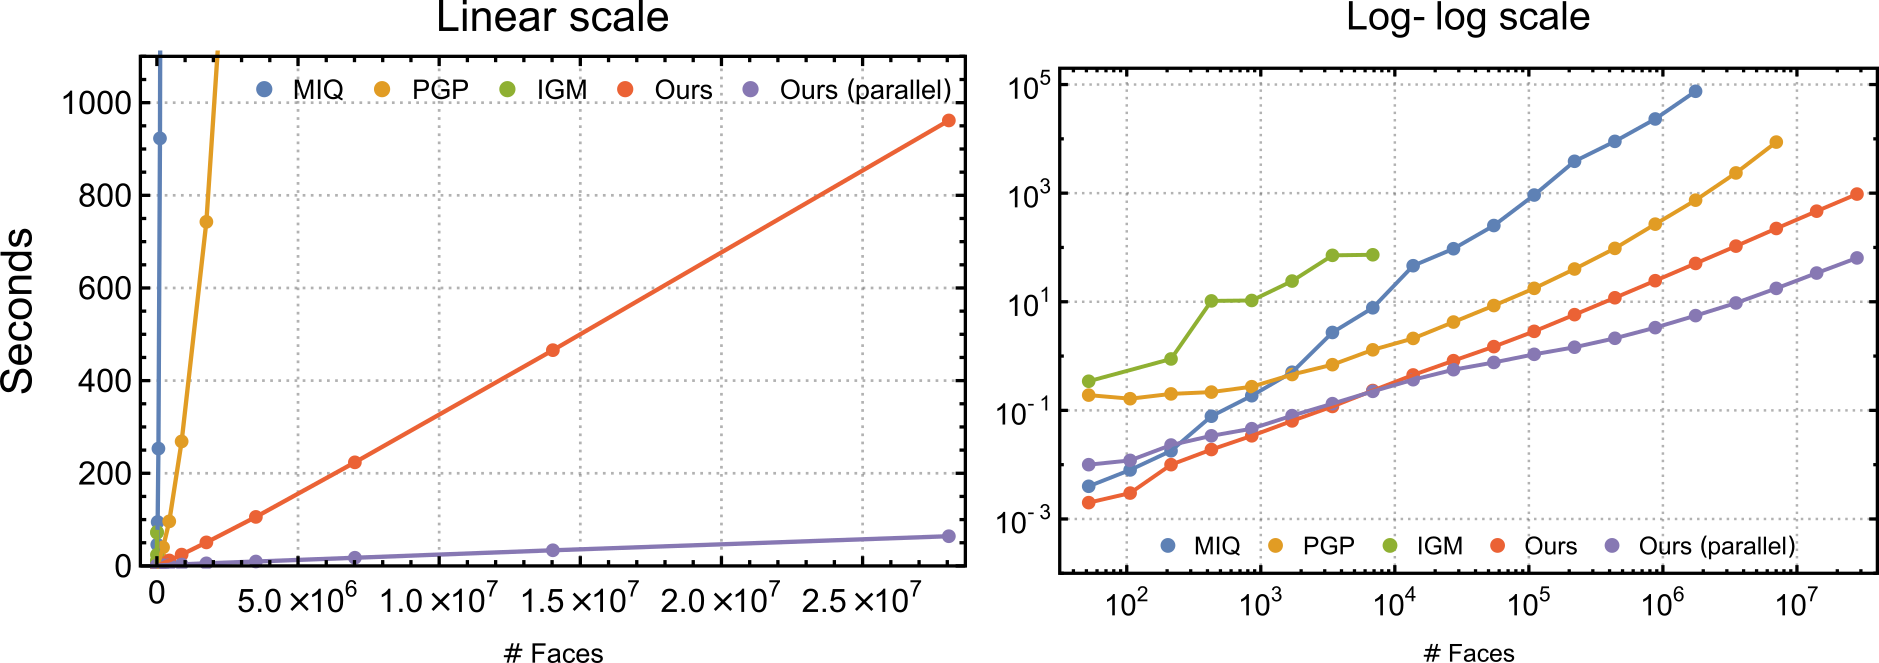
\includegraphics[width=12cm]{img/computation-time.png}\par
	\end{centering}
	\caption{Running time comparison against several global methods for a progressive input mesh. \cite{jakob2015instant}}
	\label{fig:computation-time}
\end{figure}

Current global meshing approaches yield computation times of significant superlinear growth with respect to increasing mesh sizes. In the case of MIQ (Section~\ref{MIQ}), this is mainly due to the then more complex mixed-integer problem that comes with more vertices, i.e. more and larger constraints to the problem. Solving these larger optimization problems naturally requires more time \cite{jakob2015instant,bommes2009mixed}.

Similar to other local meshing methods like PQMS (Section~\ref{PQMS}), IFAM also operates in linear time. This allows for great scalability, i.e. 3D models of incredible size can be easily quadrangulated (see Figure~\ref{fig:computation-time}). In addition, this method can be implemented in parallel, further benefiting from larger input sizes \cite{jakob2015instant}.\bigskip

This large advantage in computation time does, however, come at the cost of quality. Figure~\ref{fig:quality} illustrates the quality differences between the global approach MIQ, the local approach PQMS, and IFAM:

\begin{figure}[htb!]
	\begin{centering}
		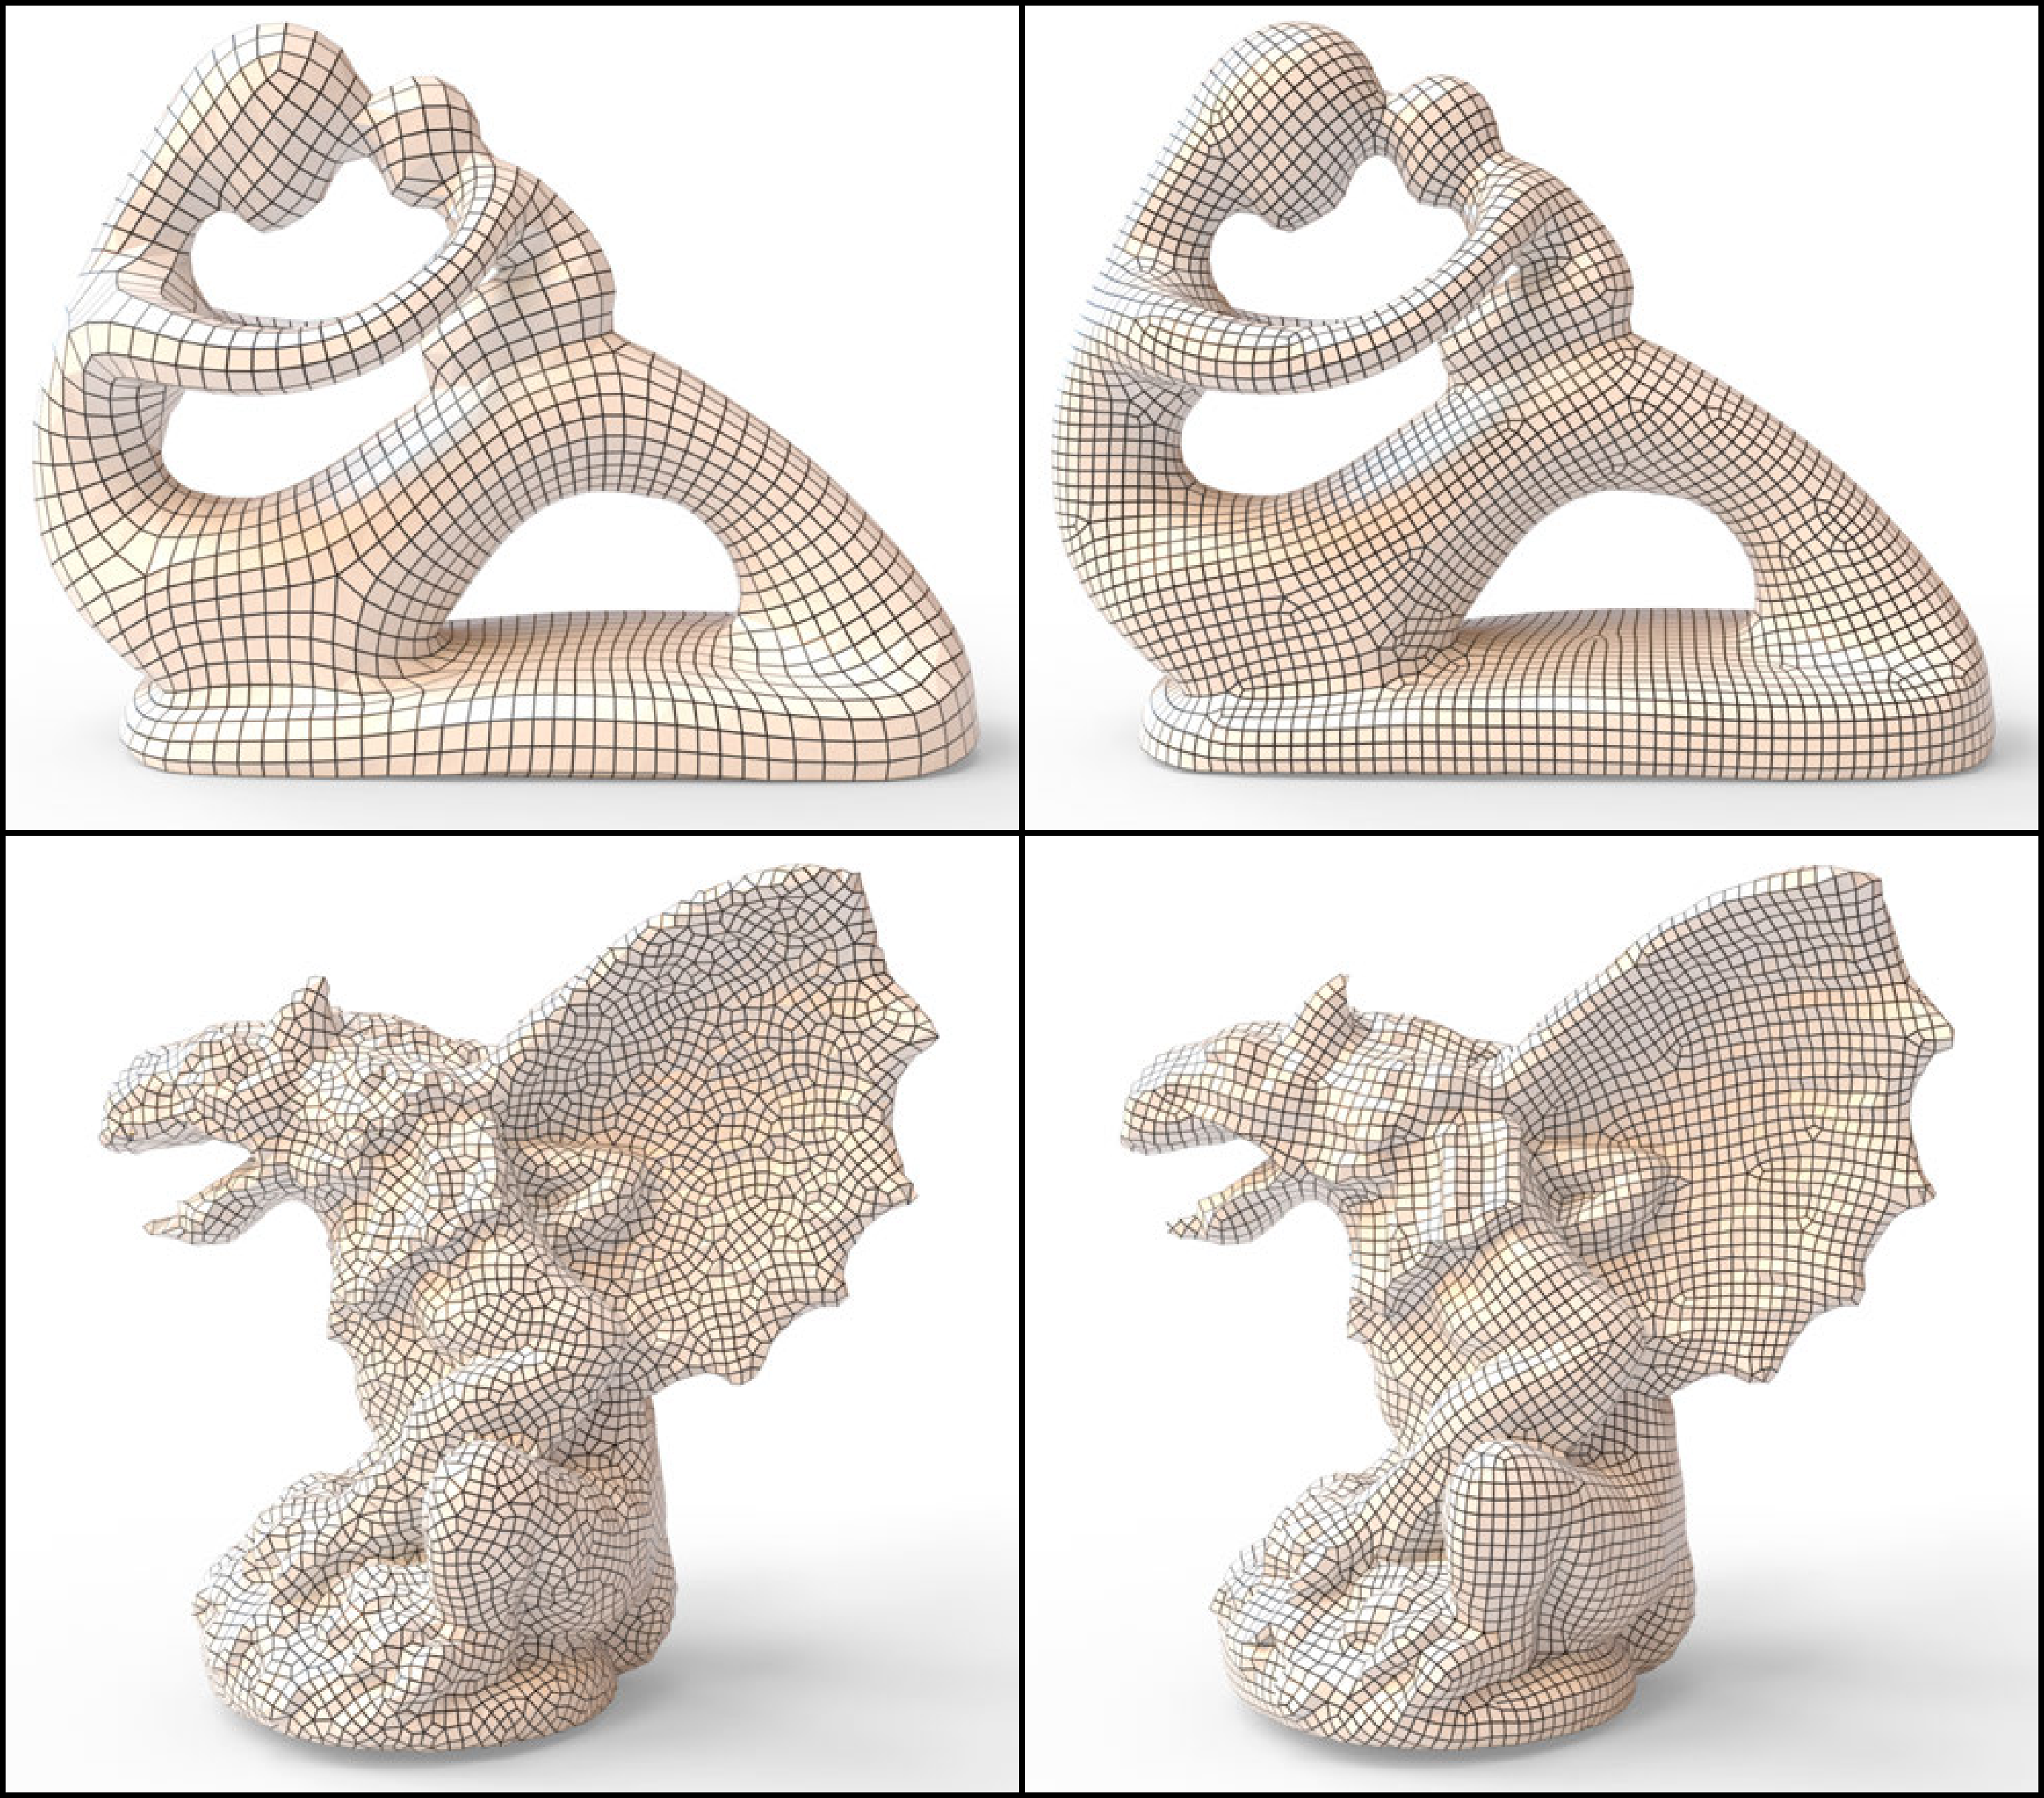
\includegraphics[width=8cm]{img/quality.png}\par
	\end{centering}
	\caption{Quadrilateral meshing comparison: MIQ \cite{bommes2009mixed} (\textit{top left}), PQMS \cite{tarini2010practical} (\textit{bottom left}), IFAM (\textit{right}). \cite{jakob2015instant}}
	\label{fig:quality}
\end{figure}

The bottom row of the Figure shows how, by making use of alignment information, the Instant Field-Aligned Meshes approach naturally snaps to shape feature, while also obtaining higher isotropy and regularity \cite{jakob2015instant}.

Compared to global approaches, IFAM lacks quality. Due to its locality, IFAM tends to create more singularities than global algorithms such as MIQ. From this comes the main point of criticism: IFAM by itself creates many singularities and singularity pairs in unexpected and unintended locations that simply would not appear in global methods. This is a problem that has yet to be dealt with. Perhaps "messy" regions in both orientation and position field, i.e. regions with high distortion, could be excluded from the output mesh, and then the resulting patches could be filled in by pattern-based patch filling such as DDIQ (Section~\ref{DDIQ}) as an optional post-processing step to minimize the occurrence of these singularity occurrences. However, as a side note, both IFAM and MIQ offer manual editing mechanisms to deal with these issues, making them both more useful for practical applications.

However, it is also evident from the top row of Figure~\ref{fig:quality} that IFAM computes are more uniform output mesh that the global method MIQ \cite{jakob2015instant}.\bigskip

Finally, local remeshing approaches are more robust to non-manifold input meshes than global methods: Even if just some regions of the mesh are non-manifold, global meshes often fail to execute and compute an output mesh. On the other hand, due to the locality of IFAM, the algorithm is mostly unaware of the existence of non-manifold regions in the input and can skip the respective vertices, thus creating an output mesh with the affected areas cut out.

%%%%%%%%%%%%%%%%%%%%%%%%%%%%%%%%%%%%%%%%%%%%%%%%%%%%%%%%%%%%
% Conclusion
\section{Conclusion}
The Instant Field-Aligned Meshes method is a robust, scalable and powerful algorithm for isotropic meshing. Its incredible efficient runtime and the ability to take different geometry representations as an input makes the algorithm very useful for practical work. However, the major limitation of an increased amount of singularities and thus lower quality compared to global methods must be addressed.\bigskip

This approach is of great interest not only to practitioners but also to researchers. The linear computation time with respect to input size is not the only attractive feature: Due to its very simple and modular construction, the three main steps of the algorithm can be used independently and modified to meet specific needs: Both the orientation- and the position-field can be incorporated into other field-aligned meshing pipelines, making way for a parameter-free method to align fields to their geometric shape. Also, the inner workings of these optimizations could be adapted, e.g. by smoothing the orientation field using vector products instead of angular differences. New work, also in related fields such as hexagonal meshing (\cite{gao2017robust}), build upon this methods' field optimizations to create improved field-aligned meshing methods. Finally, the mesh extraction method could be adjusted to work with global meshing approaches, delivering a simple solution for this task.\bigskip

Ultimately, the Instant Field-Aligned Meshes method has made a great leap in local field-aligned meshing and meshing in general. While there are still some problems to be solved, it is exciting to see what other algorithms will evolve from this.

%%%%%%%%%%%%%%%%%%%%%%%%%%%%%%%%%%%%%%%%%%%%%%%%%%%%%%%%%%%%
% Bibliography
\label{cha:references}
\printbibliography

\end{document}
